\documentclass[11pt]{article}

\usepackage{amsmath}
\usepackage{amssymb}
\usepackage[margin=0.68in]{geometry}
\usepackage{booktabs}
\usepackage{enumitem}
\usepackage{fancyhdr}
\usepackage{graphicx}
\usepackage[table]{xcolor}
\usepackage[hidelinks]{hyperref}
\usepackage{listings}
\usepackage{microtype}
\usepackage{tabularx}
\usepackage{titlesec}
\graphicspath{{docs/lessons/assets/}{../assets/}}

\definecolor{Ink}{gray}{0}
\definecolor{CodeGray}{gray}{0.96}
\hypersetup
{
    pdftitle={ADK Lesson 027: Multi-Source Telemetry Console},
    pdfauthor={Kevin Shanahan},
    pdfsubject={Deterministic source health, operator acknowledgement, presentation, and bounded records},
    pdflang={en-US}
}
\pagestyle{fancy}
\fancyhf{}
\lhead{\textsc{ADK Lesson 027}}
\rhead{Multi-Source Telemetry Console}
\cfoot{\thepage}
\setlength{\headheight}{14pt}
\setlength{\parindent}{0pt}
\setlength{\parskip}{5pt}
\setlist{nosep,leftmargin=1.45em}
\titleformat{\section}{\Large\bfseries\color{Ink}}{\thesection}{0.5em}{}
\titleformat{\subsection}{\large\bfseries\color{Ink}}{\thesubsection}{0.5em}{}
\lstdefinestyle{adkcpp}
{
    language=C++,
    backgroundcolor=\color{CodeGray},
    basicstyle=\ttfamily\small,
    keywordstyle=\color{Ink}\bfseries,
    commentstyle=\color{Ink},
    columns=fullflexible,
    keepspaces=true,
    showstringspaces=false,
    frame=single,
    rulecolor=\color{Ink},
    breaklines=true,
    tabsize=4
}
\newcommand{\checkbox}{\(\square\)}
\newcommand{\blank}[1]{\rule{#1}{0.4pt}}
\newcommand{\lessonbox}[1]{%
  \begin{center}
  \fcolorbox{Ink}{white}{\parbox{0.92\linewidth}{#1}}
  \end{center}}

\begin{document}

\begin{center}
  {\Huge\bfseries Multi-Source Telemetry Console}\\[4pt]
  {\Large Preserve health evidence across presentation and records}\\[8pt]
  \textit{A deterministic, receive-only project with no actuator}
\end{center}

\begin{tabularx}{\linewidth}{@{}>{\bfseries}l X >{\bfseries}l X@{}}
Lesson & 027 --- project & Time & 240--330 minutes\\
Prerequisites & Lessons 001--026 & Board & Arduino Mega 2560\\
Evidence & RGB cadence and D13 & Status & host verification; bench open\\
Energy class & E1: USB, passive buttons, resistor-limited LEDs\\
\end{tabularx}

\lessonbox{\textbf{Boundary.} This is an educational annunciator for owned lab
fixtures. It is not a fire, burglar, medical, industrial, environmental-safety,
or emergency system. It does not actuate anything, dispatch help, transmit,
replay, clone, or interpret an unknown protocol.}

\section{Mission and evidence chain}

Compose the receive-only arc without losing the distinction between evidence
and presentation:
\[
\text{source evidence}\rightarrow\text{normalized reading}\rightarrow
\text{console decision}\rightarrow\text{visible state}\rightarrow
\text{stable record}.
\]

The released exercise uses three compiled-in, owned fixture observations:
temperature, relative humidity, and contact. A live receiver is not required.
Input order cannot change configured source order. Missing sources remain
explicit. Presentation and record failures cannot rewrite health.

\begin{center}
% ADK visual: pencil
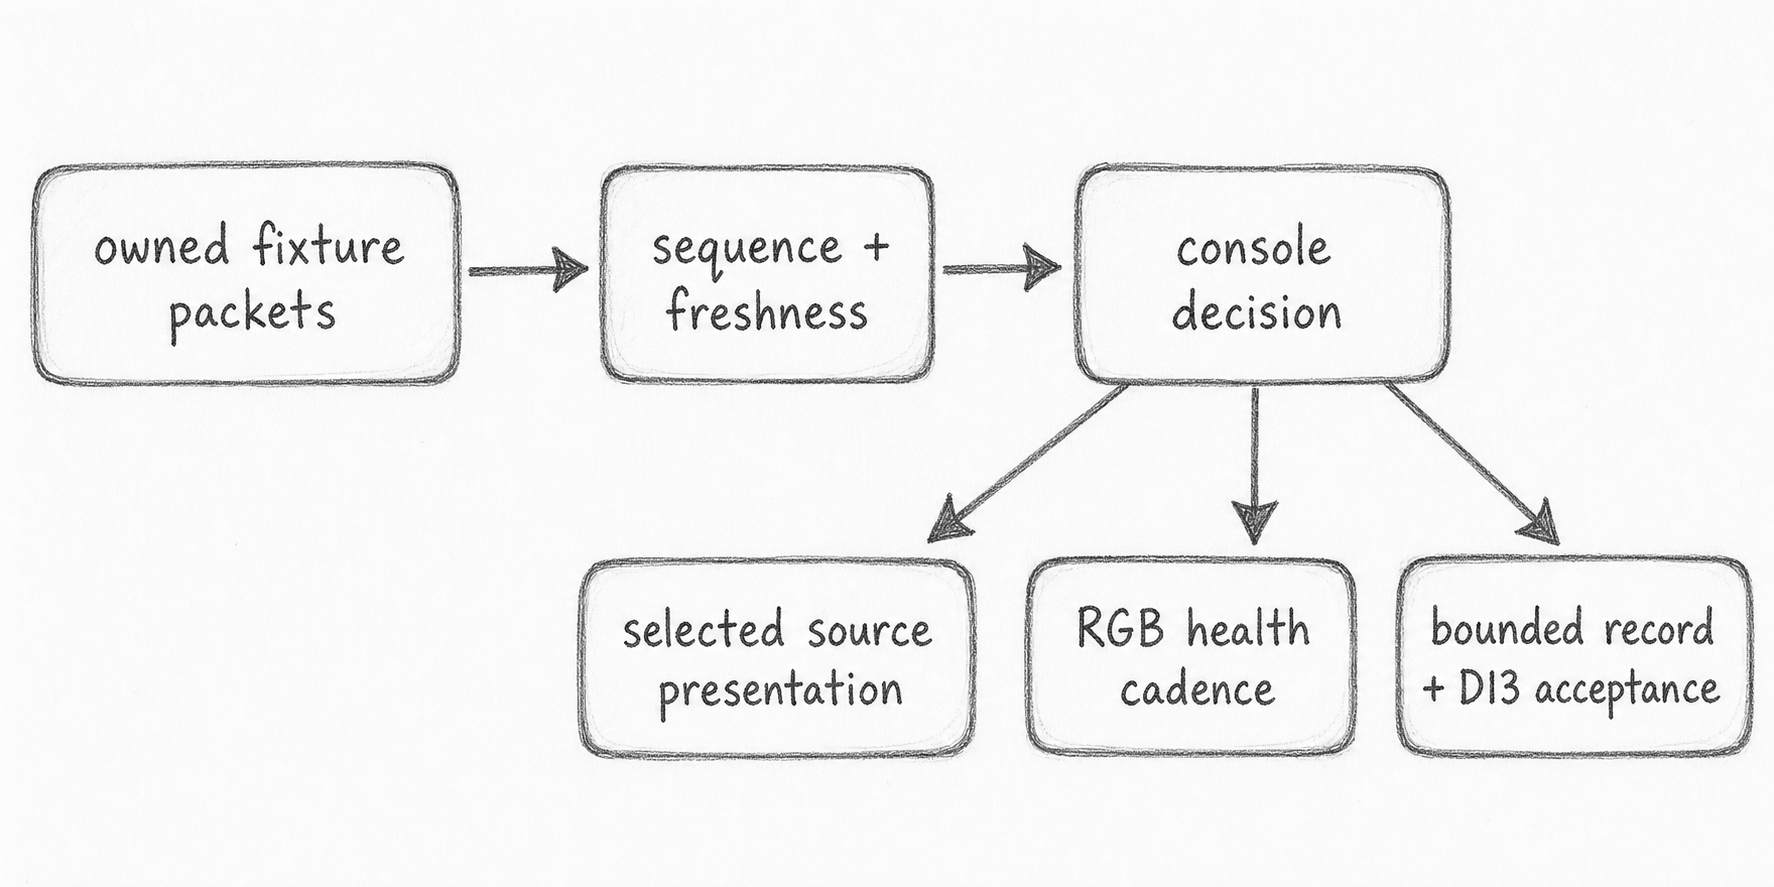
\includegraphics[width=0.96\linewidth]{027-evidence-chain-pencil.png}
\end{center}

\subsection{Learning outcomes}

\begin{itemize}
  \item distinguish capture, frame, packet, record, and presentation;
  \item explain configured slot order and explicit missing observations;
  \item derive health from quality, sequence condition, and freshness;
  \item keep acknowledgement separate from health;
  \item prove record acceptance without confusing it with source validity;
  \item replay an exact mixed-source trace with byte-identical output.
\end{itemize}

\section{Orientation and circuit plan}

\begin{center}
% ADK visual: pencil
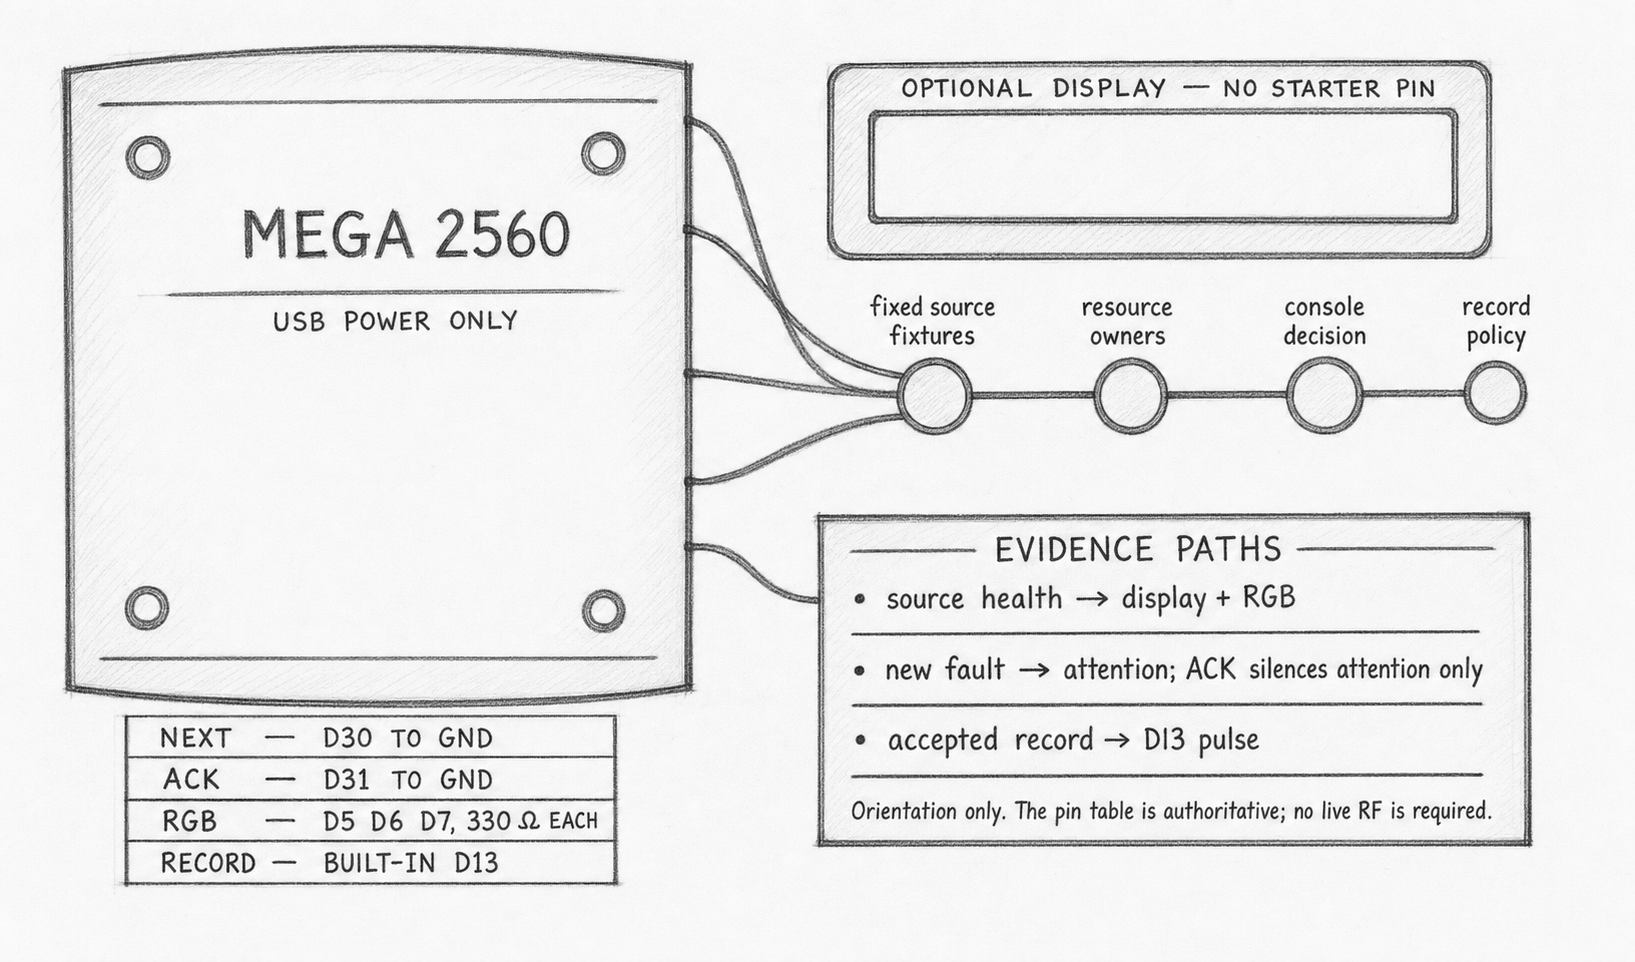
\includegraphics[width=0.96\linewidth]{027-telemetry-console-pencil.png}

\small\textit{Alternative text: graphite orientation plate showing the
USB-powered Mega, optional unassigned display, D30 next and D31 acknowledge
buttons to ground, D5--D7 RGB channels with one 330-ohm resistor each, built-in
D13 record evidence, and separate health and record paths. No live radio or
actuator is shown.}
\end{center}

The plate shows the extension path as well as the starter circuit. The released
sketch's pin table below is authoritative; the display block is optional
further work and owns no pin in the starter circuit.

\begin{tabularx}{\linewidth}{@{}l X X@{}}
\toprule
Circuit element & Released role & Electrical constraint\\
\midrule
Next button, D30 & advance configured source slot & internal pull-up; switch to GND\\
Acknowledge button, D31 & acknowledge current attention intent & internal pull-up; switch to GND\\
RGB LED, D5--D7 & health plus non-color cadence & one 330 ohm resistor per channel\\
D13 LED & toggles after complete record acceptance & built-in LED, independent of health\\
Source fixtures & deterministic observation evidence & compiled-in, owned lab values\\
\bottomrule
\end{tabularx}

\textbf{Unpowered prediction.} Circle every resource owner in the final sketch.
For each borrower, draw an arrow to the owner that must outlive it. Confirm
button wiring, one resistor per RGB channel, common ground, and no display,
sounder, relay, external load supply, transmitter, or mains connection.

\section{Vocabulary worksheet}

\begin{tabularx}{\linewidth}{@{}l X X@{}}
\toprule
Word & Meaning in this arc & What it does not mean\\
\midrule
Capture & timestamped physical evidence & decoded command\\
Frame & bounded protocol candidate & trusted packet\\
Packet & ADK-owned telemetry envelope & authenticated identity\\
Record & stable storage representation & source truth\\
Presentation & human-visible interpretation & mutation of observation health\\
\bottomrule
\end{tabularx}

CRC detects accidental corruption. It does not authenticate a sender, hide
content, prove a location, or prevent replay. Source identifiers organize owned
fixtures; they are not credentials. Freshness bounds local age; it does not
prove a remote clock.

\section{The narrative loop}

\begin{lstlisting}[style=adkcpp]
observeTelemetrySources (now);
decideConsoleState      (now);
presentConsoleState     (now);
recordConsoleEvidence   (now);
\end{lstlisting}

\texttt{observe} builds the fixed observation fixture. \texttt{decide} submits
one complete configured-slot view through \texttt{TelemetryConsoleProject}.
\texttt{present} checks the RGB presentation result. \texttt{record} checks
the bounded record result. No stage hides time or allocates memory.

\subsection{Object-order exercise}

Number these in construction order: \blank{.25in} console,
\blank{.25in} runtime, \blank{.25in} project,
\blank{.25in} fixture observations, \blank{.25in} buttons,
\blank{.25in} record sink, \blank{.25in} RGB presentation.

Then answer:

\begin{enumerate}
  \item Which object decides source health? \blank{2.4in}
  \item Which object decides whether one stable record is pending? \blank{2.1in}
  \item Which failure may silence a cue without changing health? \blank{2.0in}
  \item Why is packet arrival order excluded from source selection?
        \blank{2.5in}
\end{enumerate}

\section{Health precedence}

\begin{tabularx}{\linewidth}{@{}l X X@{}}
\toprule
Health & Required interpretation & Evidence\\
\midrule
Starting & expected slots have not all produced usable observations & blue cadence\\
Healthy & every expected slot is present, valid quality, and fresh & green cadence\\
Degraded & an observation is aging or reports a sequence gap & amber cadence\\
Fault & stale, invalid, corrupt, duplicate, or missing evidence & fast red cadence\\
Stopped & lifecycle inactive & unlit\\
\bottomrule
\end{tabularx}

Fault dominates degraded; degraded dominates healthy; startup is not silently
healthy. When several conditions coexist, the same input snapshot must always
choose the same result.

\subsection{Precedence worksheet}

\begin{tabularx}{\linewidth}{@{}X l l l@{}}
\toprule
Input set & Prediction & Observation & Interpretation\\
\midrule
all valid/fresh & \blank{.7in} & \blank{.7in} & \blank{1.3in}\\
one aging + one gap & \blank{.7in} & \blank{.7in} & \blank{1.3in}\\
one stale + one aging & \blank{.7in} & \blank{.7in} & \blank{1.3in}\\
duplicate identity & \blank{.7in} & \blank{.7in} & \blank{1.3in}\\
missing configured slot & \blank{.7in} & \blank{.7in} & \blank{1.3in}\\
\bottomrule
\end{tabularx}

\section{Operator intent is not evidence}

The next action selects a configured slot, not a source ID or packet-arrival
position. A held button produces one debounced event. Selection wraps after
the last configured slot.

Acknowledgement applies only to the current attention intent. The starter
circuit has no sounder; inspect the state in host replay, then add a bounded
sounder only as the extension exercise. Acknowledgement does not:

\begin{itemize}
  \item convert fault to healthy;
  \item clear a missing or stale source;
  \item erase or rewrite a record;
  \item prevent a new fault from being announced.
\end{itemize}

\textbf{Experiment.} Enter fault, acknowledge it, and keep the fault present.
Predict fast red evidence will remain. Inspect the replay snapshot to see
\texttt{Attention} become \texttt{Notice}. Recover, then introduce a new fault
and predict \texttt{Attention} again.

\section{Presentation and record separation}

The released presentation converts health to an RGB color and a distinct
cadence. Its selected-source argument stays available for a later display
without entering the decision. A presentation failure leaves the source
snapshot unchanged.

The record policy writes on accepted observation, health transition,
acknowledgement, or periodic heartbeat. Simultaneous reasons become one record
under fixed priority. A failed write remains visible and may retry only under a
bounded deterministic policy. No queue grows in SRAM.

\begin{tabularx}{\linewidth}{@{}l X X@{}}
\toprule
Failure & Must remain unchanged & Separate evidence\\
\midrule
presentation write & source health and pending record & returned status\\
record append & source health and selected slot & D13 does not toggle\\
record retry & accepted observation snapshot & same bounded record bytes\\
attention extension & health and record intent & red evidence remains\\
\bottomrule
\end{tabularx}

\subsection{Golden-record worksheet}

Copy one released canonical record exactly:

\vspace{0.2in}
\hrule
\vspace{0.2in}
\hrule

\begin{tabularx}{\linewidth}{@{}l X@{}}
Trigger reason & \blank{3.4in}\\
Caller capacity & \blank{1.0in} bytes\\
Encoded size & \blank{1.0in} bytes\\
First differing byte after corruption & \blank{1.2in}\\
Retry byte-identical? & yes / no; evidence: \blank{2.0in}\\
\end{tabularx}

\section{Deterministic replay lab}

Prepare one exact trace:

\begin{enumerate}
  \item start with all three slots missing;
  \item recover temperature, humidity, then contact in configured order;
  \item deliver later packets in a different arrival order;
  \item age one source to the exact degraded boundary;
  \item cross the stale boundary;
  \item acknowledge attention while fault remains;
  \item recover, then introduce a different fault;
  \item inject one record failure and bounded retry;
  \item shut down from the active fault state.
\end{enumerate}

\begin{tabularx}{\linewidth}{@{}r l l l l@{}}
\toprule
Time & Source change & Expected health & Selected slot & Record reason\\
\midrule
\blank{.5in} & all missing & \blank{.8in} & \blank{.5in} & \blank{.9in}\\
\blank{.5in} & first recovery & \blank{.8in} & \blank{.5in} & \blank{.9in}\\
\blank{.5in} & all recovered & \blank{.8in} & \blank{.5in} & \blank{.9in}\\
\blank{.5in} & exact aging & \blank{.8in} & \blank{.5in} & \blank{.9in}\\
\blank{.5in} & exact stale & \blank{.8in} & \blank{.5in} & \blank{.9in}\\
\blank{.5in} & acknowledge & \blank{.8in} & \blank{.5in} & \blank{.9in}\\
\bottomrule
\end{tabularx}

Replay the same timestamps, packet bytes, and button events twice. Compare
health, signal intent, selected slot, record reasons, and record bytes. Every
difference is a failure until explained.

\section{Predict, observe, interpret}

\subsection{Resource acquisition}

\textbf{Predict:} blue cadence appears only after all required owners
initialize. \textbf{Observe:} startup cadence without Serial.
\textbf{Interpret:} this supports resource acquisition; it does not prove
shutdown release or a valid source.

\subsection{Source health}

\textbf{Predict:} the trace advances blue, green, amber, red.
\textbf{Observe:} the RGB cadence at TP-R, TP-G, and TP-B.
\textbf{Interpret:} agreement supports the console decision. It does not
authenticate a fixture or establish sensor accuracy.

\subsection{Record acceptance}

\textbf{Predict:} D13 toggles only after a complete record is accepted.
\textbf{Observe:} inject a failed append in the host fixture and compare the
acceptance state with health evidence.
\textbf{Interpret:} D13 proves the simulated storage call path, not physical
media durability.

\subsection{Safe shutdown}

\textbf{Predict:} RGB and record evidence become inactive and owned pins
release. \textbf{Observe:} measure D5--D7 and D13 against GND after the stop
path. \textbf{Interpret:} inactive LEDs alone do not prove high impedance or
claim release.

\section{Diagnosis}

\begin{tabularx}{\linewidth}{@{}l X@{}}
\toprule
Observation & Check in order\\
\midrule
stays Starting & configured count, explicit presence, first observation time\\
Fault instead of Degraded & stale boundary, invalid quality, duplicate ID, missing slot\\
selection follows arrival & configured-slot table; never sort by packet arrival\\
acknowledgement clears red & separate sound acknowledgement from health state\\
D13 toggles on failed record & acceptance must follow a successful append\\
new fault lacks attention & fault-episode transition and acknowledgement reset\\
different second replay & hidden clock, mutable fixture, uninitialized padding, ordering\\
\bottomrule
\end{tabularx}

\section{CLI workflow and acceptance}

\begin{lstlisting}[style=adkcpp]
make host-test
make host-test-sanitize
make telemetry-fixtures-check
make arduino-Lesson027TelemetryConsole
make size-Lesson027TelemetryConsole
make lessons
make lessons-check
make site-check
make upload EXAMPLE=Lesson027TelemetryConsole PORT=/dev/ttyACM0
make hardware-card LESSON=027 BOARD=mega2560
\end{lstlisting}

These targets verify code and publication, not the open physical card. There is
intentionally no transmit, replay, clone, brute-force, scan, or protocol-export
target.

\subsection{Unsigned physical acceptance card}

\begin{itemize}
  \item \checkbox\ Exact Mega revision, buttons, LEDs, supply, and instrument
        recorded.
  \item \checkbox\ Wiring and resistor values checked with USB removed.
  \item \checkbox\ Startup acquisition evidence observed.
  \item \checkbox\ Healthy, degraded, fault, acknowledgement, reannouncement,
        and recovery evidence observed.
  \item \checkbox\ Record failure kept separate from source health.
  \item \checkbox\ Shutdown output state measured at named test points.
  \item \checkbox\ No transmitter, actuator, relay, external load, or mains
        circuit present.
\end{itemize}

\begin{tabularx}{\linewidth}{@{}l X@{}}
Board and revision & \blank{3.8in}\\
Exact specimens and markings & \blank{3.2in}\\
Supply and instruments & \blank{3.45in}\\
Firmware commit and tool versions & \blank{2.65in}\\
Predictions & \blank{4.45in}\\
Observations & \blank{4.35in}\\
Interpretation and deviations & \blank{3.25in}\\
Operator and date & \blank{3.8in}\\
\end{tabularx}

\lessonbox{\textbf{Open gate.} Host replay, firmware compilation, a generated
PDF, and visual inspection are not physical verification. Leave this card
blank until the released circuit is measured on a Mega 2560.}

\section{Further work}

\begin{enumerate}
  \item Add a fourth generated source without changing arrival-order behavior.
  \item Design an explicit log-full policy with no heap and no silent overwrite.
  \item Explain what cryptographic authentication would require and why CRC,
        source ID, sequence, and freshness do not provide it.
  \item Add a bounded sounder for attention while retaining the RGB state as
        equivalent non-audible evidence.
  \item Audit the final object graph for ownership, rollback, shutdown order,
        and exception-unwinding safety in a caller.
\end{enumerate}

\section*{Package status}

The interface, deterministic host tests, canonical Mega sketch, and printable
package are present. Physical Mega acceptance remains open. The exercise makes
no live-radio or multi-room hardware claim.

\end{document}
